\documentclass{proc}

\usepackage{hyperref}
\usepackage{listings}
\usepackage{graphicx}
\usepackage{float}

\newcommand{\noun}[1]{\textsc{#1}}

\begin{document}

\title{Concepts tool - Manual}
\author{Jonathan Beaumont\\
\texttt{j.r.beaumont@ncl.ac.uk}\\
\emph{School of Electrical and Electronic Engineering, Newcastle University,UK}\\\\
Last updated \today}

\maketitle

\tableofcontents

\onecolumn

\section{Introduction}

\emph{Concepts} are a formal method of specifying asynchronous circuits. With concepts, one can describe behaviours of a circuit and its environment at various levels, with the aim of
defining the behaviours in terms of gates, protocols or simple signal interactions. Using this method, one can split a design into scenarios, based on operational modes, individual functions, or 
any other method a user decides. These can be specified separately, using concepts, and then combined to provide a full system specification. Through this, reuse is promoted,
 allowing concepts to be reused between scenarios and even entire designs. More information on the theory of concepts can be found in~\cite{2016_beaumont_concepts}, the latest version 
of which can be found \href{https://github.com/tuura/concepts-article/releases}{here}.

In this document, we will discuss the associated tool for concepts. This open source tool is written in \emph{Haskell}, and contains both the library for concepts, 
including abstract concepts and circuit concepts built upon the abstract, and a tool for translating concepts into \emph{Signal Transition Graphs}~(STGs)~\cite{Chu_1987_phd}
\cite{Rosenblum_1985_tpn}. These are commonly used for the specification, verification and synthesis of asynchronous control circuits in the academic community, and they are supported 
by multiple EDA tools, such as \noun{Petrify}~\cite{Cortadella},\noun{Mpsat}~\cite{khomenko2004detecting}, \noun{Versify}~\cite{i1997formal},\noun{Workcraft}~
\cite{2007_poliakov_workcraft}\cite{Workcraft_website}, and others.  The aim of this tool is to design and debug concepts, and then translate them to STGs, where they can be used with
 these tools. 

The latest version of this tool, and this manual, can be found \href{https://github.com/tuura/concepts}{in the GitHub repo}. This tool is also distributed as a back-end tool for 
\noun{Workcraft}. This version of the concepts tool will be the latest version that works correctly with \noun{Workcraft}. The latest version of \noun{Workcraft}, which also features tools 
 such as \noun{Petrify} and \noun{Mpsat}, can be downloaded from \url{http://workcraft.org/}. 

\section{Installation}

The concepts tool, as well as \noun{Workcraft} are available for \emph{Windows}, \emph{Linux} and \emph{Mac OS X}. The installation instructions for all of these operating systems are 
the same. We will be referring to directories using the forward-slash character ('/') as a separator, however for \emph{Windows}, replace this with a back-slash character 
('\textbackslash').

If choosing to use the concepts tool on its own, this must be 
downloaded from the \href{https://github.com/tuura/concepts}{GitHub repo}. If you choose to use this tool as part of \noun{Workcraft}, download this from the 
\href{http://workcraft.org/}{\noun{Workcraft} website}. Once downloaded, extract the contents of the folder, and move them to a directory you wish to run them from. 

\subsection{Concepts tool requirements\label{sub:Concepts_requirements}}

The concepts tool is written in \emph{Haskell}, and as such, the \emph{Glasgow Haskell Compiler}~(GHC) is required for installation as well as the \emph{Cabal} library builder. 
Cabal builds and installs packages for Haskell, and is necessary for the concepts tool. GHC and Cabal can be downloaded from \url{https://haskell.org/downloads}. We recommend the
 "Minimal installers", as this contains GHC and Cabal.

If needed, download the installers for GHC and Cabal, and follow the instructions to install these.

\subsection{Workcraft requirements}

\noun{Workcraft} is written in Java, and the latest version of the \emph{Java Runtime Environment}~(JRE) needs to be installed to run.  This can be downloaded from 
\url{http://java.com/en/download/}. 

If needed, download the JRE installer, and follow the instructions to install this.

While the concepts tool is distributed with \noun{Workcraft}, it still needs to be built by Cabal in order for it to be run. 
See Section~\ref{sub:Concepts_requirements} for requirements for the concepts tool.

\newpage
\subsection{Installing the tool}

Once either the concepts tool or \noun{Workcraft} has been extracted and moved to the desired directory, using command line, navigate to the concepts tool directory, or if using 
\noun{Workcraft}, navigate to this directory, and then navigate to the concepts tool directory, found in \texttt{tools/concepts} (for \emph{OS X}, it is located within the \texttt{Workcraft.app} contents folder \texttt{Contents/Resources/tools/concepts}.

Now, the process of installing the tool is the same, regardless of how you aim to use the concepts tool. First of all, let's update the Cabal package list. To do this, run: 

\begin{lstlisting}[language=bash]
  $ cabal update
\end{lstlisting}

When this has finished, the package list will be updated, and all dependencies of the concepts tool will be able to be automatically downloaded, built and installed during the process of 
installing the concepts tool.

Now, to build and install the concepts tool, simply run:

\begin{lstlisting}[language=bash]
  $ cabal install
\end{lstlisting}

If this process completes successfully, the tool will now be installed and ready to be used.

\section{Using the tool from command line}

With the tool installed, we can now start to use it to translate concepts to STGs. We will begin by discussing how it is used from command line. Usage as a back-end tool in 
\noun{Workcraft} is discussed in Section~\ref{sec:workcraft_usage}.

The standard command for the tool is as follows:

\begin{lstlisting}[language=bash]
  $ runghc <path-to-translate> <path-to-concepts-file>
\end{lstlisting}

The three parts of this are as follows:
\begin{itemize}
  \item \texttt{runghc} - This runs the translate file
  \item \texttt{<path-to-translate>} - This is file path pointing to the translate code file, which performs the necessary operations to translate concepts to STGs.
  \item \texttt{<path-to-concepts-file>} - This is the path pointing to the file containing the concepts to be translated.
\end{itemize}

When running the concepts tool from command line, it does not necessarily matter in which directory you currently are, as long as the paths to the translate code, and the concepts
file are correct.  

Now, let's use one of the examples included with the concepts tool to show the usage. These can be found in the \texttt{examples} directory. For this section, we will assume that we are 
currently in the concepts tool directory. The example we will use is the file titled "\texttt{Celement\_with\_env\_1.hs}". This has the ".hs" file extension, as it is in fact a file using Haskell 
code, and all files containing concepts should feature this file extension. To translate this concepts file to an STG, the following command must be run:

\begin{lstlisting}[language=bash]
  $ runghc translate/Main.hs examples/Celement_with_env_1.hs
\end{lstlisting}

When the translation is complete, the tool will output the following:

\begin{lstlisting}[language=bash]
  .model out
  .inputs A B
  .outputs C
  .internals
  .graph
  A0 A+
  A+ A1
  A1 A-
  A- A0
  B0 B+
  B+ B1
  B1 B-
  B- B0
  C0 C+
  C+ C1
  C1 C-
  C- C0
  A1 C+
  C+ A1
  B1 C+
  C+ B1
  C1 A-
  A- C1
  C1 B-
  B- C1
  A0 C-
  C- A0
  B0 C-
  C- B0
  C0 A+
  A+ C0
  C0 B+
  B+ C0
  .marking {A0 B0 C0}
  .end
\end{lstlisting}

This output is the STG representation in \emph{.g} format. \emph{.g} files are a standard type used as input to tools, such as \noun{Petrify}, \noun{Mpsat}, and \noun{Workcraft}. 
Therefore, this output can by copy-and-pasted into a file, and saved with the file etension \emph{.g}, and then used as input to these tools. 

The concepts tool can be used in a similar way, ensuring that the file paths to the translate code file, and the concepts input file, are correct. Section~\ref{sec:concepts_layout} contains 
information on how to layout a concepts file, to avoid as many errors as possible. 

Any errors that occur during the translation process will produce errors referring to the problematic areas, usually lines, of the concepts that are problematic. 

\section{Using the tool from \noun{Workcraft} \label{sec:workcraft_usage}}

This section will discuss how to use the concepts tool from within \noun{Workcraft}. There are many other features of \noun{Workcraft}, both as part of the STG plug in, some of which I
 will discuss in the context of concepts here, and as part of other modelling formalisms. More information on these can be found at \url{http://workcraft.org/}.
 
 \subsection{Translating and authoring concepts}

First of all, \noun{Workcraft} must be started. This can be done by running the start up script, located in the \noun{Workcraft} directory in \emph{Windows} and \emph{Linux}. In 
\emph{Windows}, this script is named ``\texttt{workcraft.bat}". In \emph{Linux}, it is simply "\texttt{workcraft}". In \emph{OS X}, \noun{Workcraft} can be started instead by double 
clicking the \noun{Workcraft} icon, which is the app container for the necessary files. 

When workcraft starts, you will be greeted by blank screen, as seen in Figure~\ref{fig:blank_workcraft_screen}.

\begin{figure}[H]
\begin{centering}
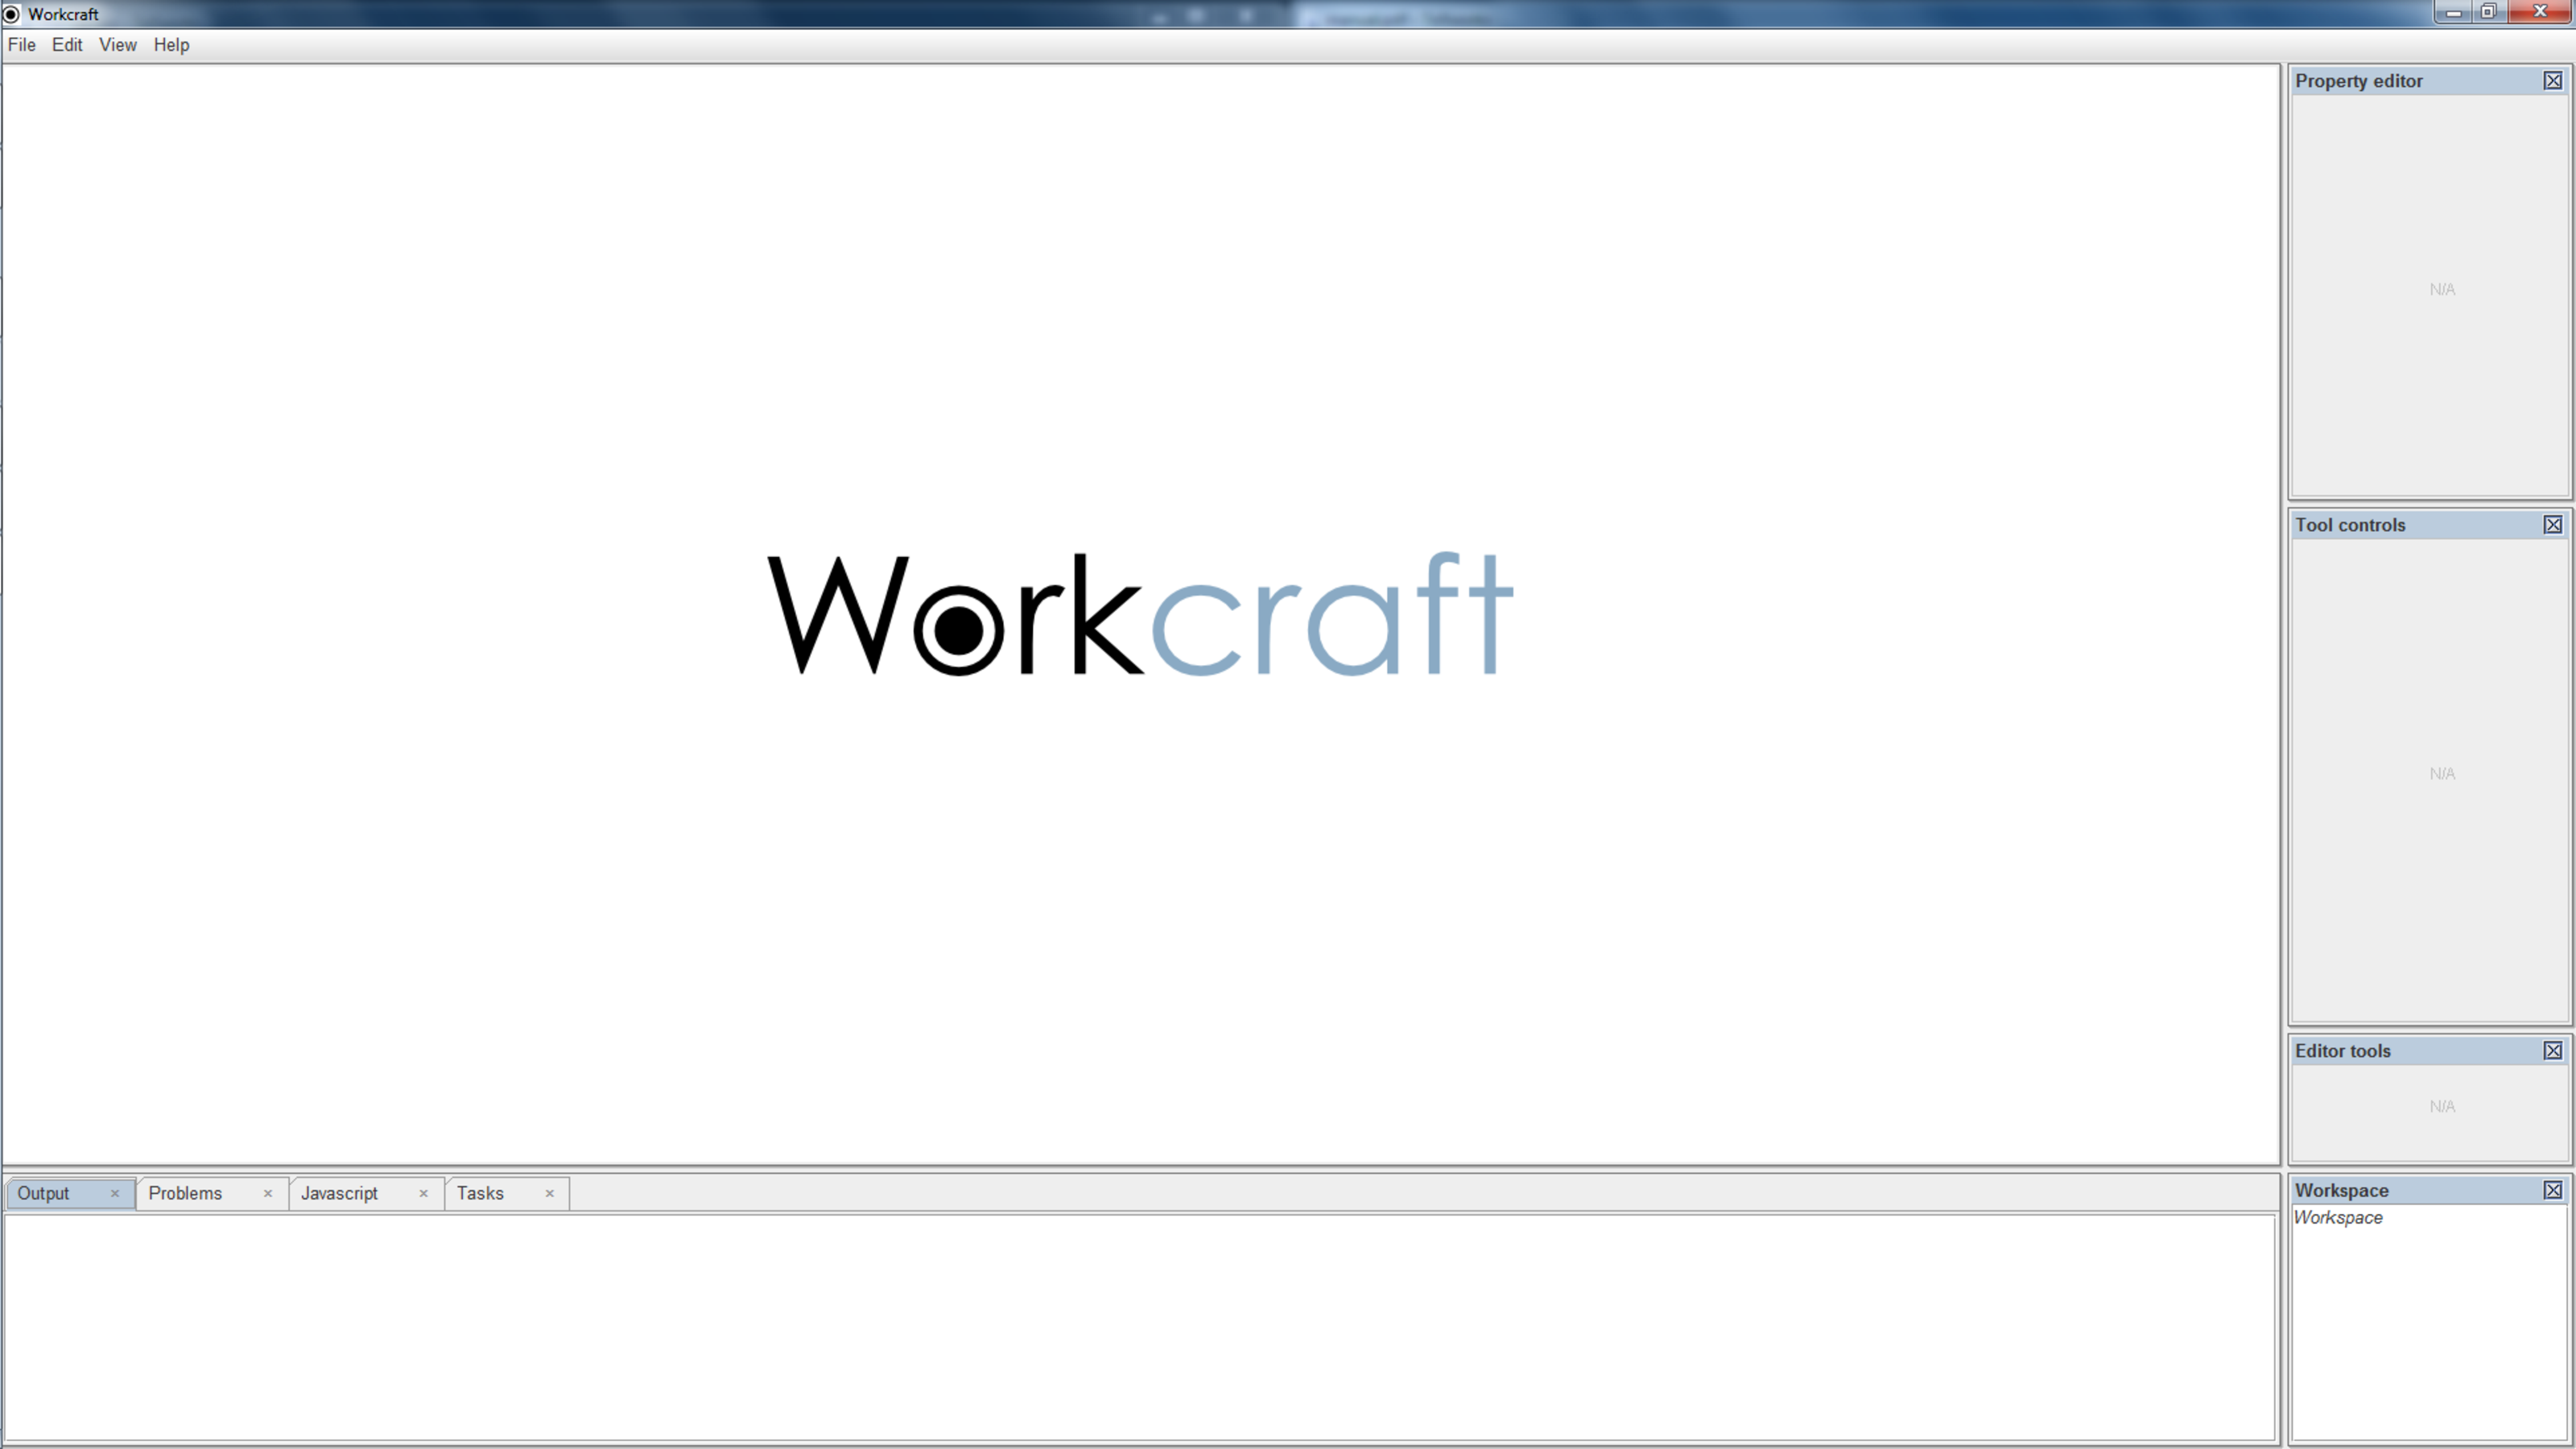
\includegraphics[scale=0.2]{images/blank_workcraft_screenshot}
\par\end{centering}

\begin{centering}
\protect\caption{\label{fig:blank_workcraft_screen}Workcraft immediately after starting.}

\par\end{centering}

\end{figure}

Now, we need to open a new work, specifically a new STG work. Open the "New work" dialog using the menu bar, \texttt{File -> Create work...}, or by pressing \texttt{Ctrl-N} 
(\texttt{CMD-N} on \emph{OS X}). This will bring up a menu as seen in Figure~\ref{fig:new_work_screen}.

\begin{figure}[H]
\begin{centering}
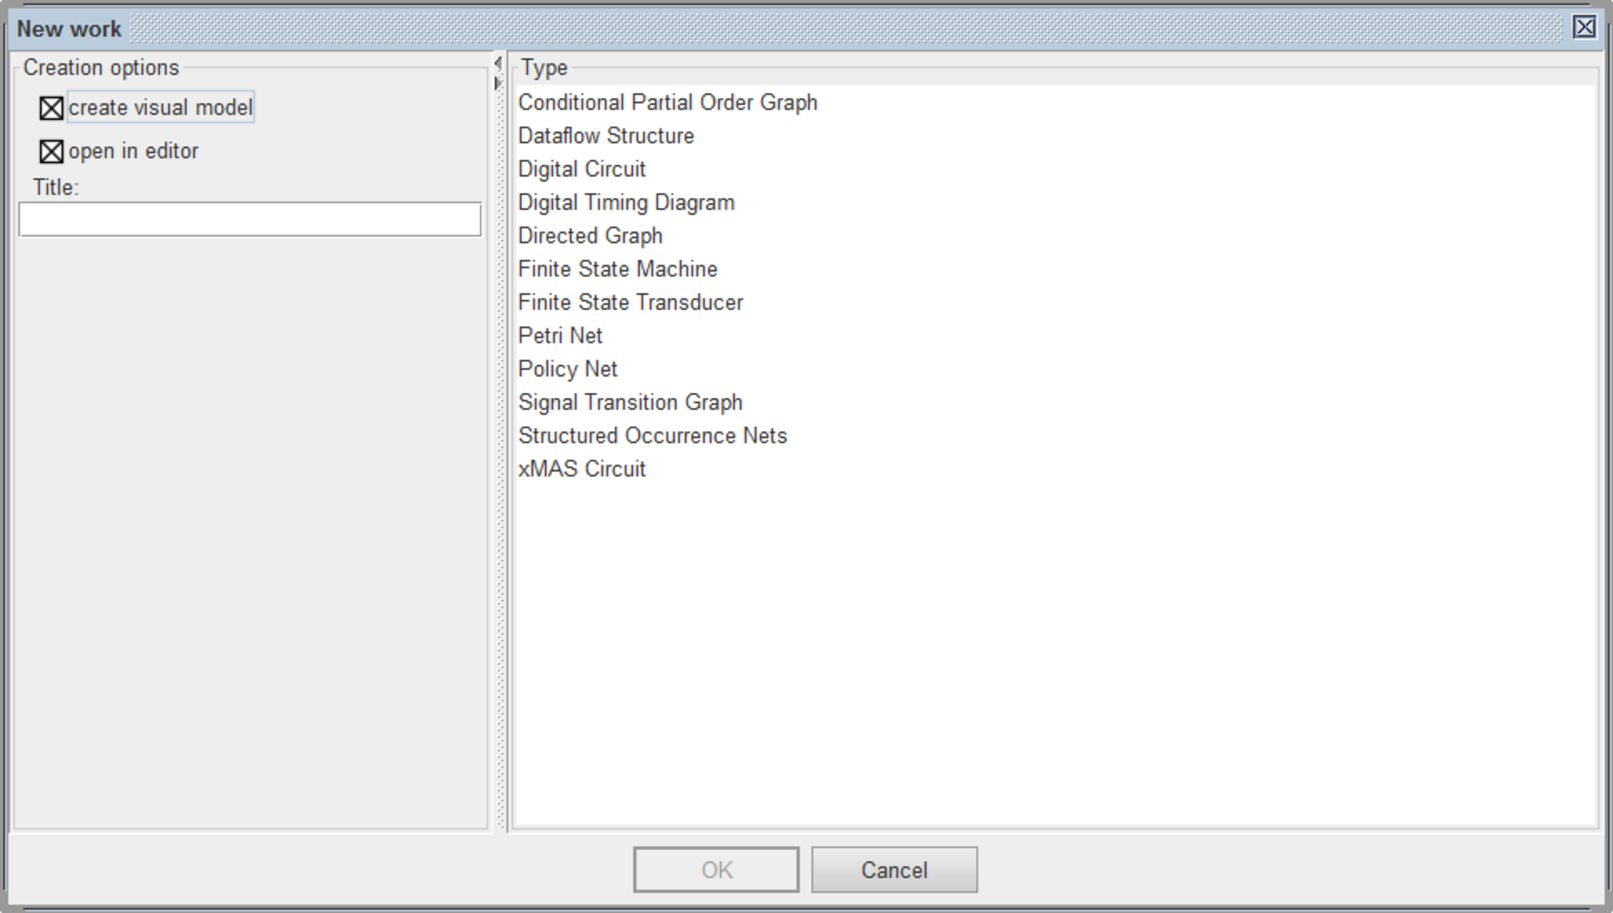
\includegraphics[scale=0.4]{images/new_work_screenshot}
\par\end{centering}

\begin{centering}
\protect\caption{\label{fig:new_work_screen}The create work window.}

\par\end{centering}

\end{figure}

In this window, select ``\emph{Signal Transition Graph}' abd cick the ``OK'' button at the bottom of the window. This will the open a blank workspace in which we can create an STG, which 
will look similar to Figure~\ref{fig:blank_stg_work}.

\begin{figure}[H]
\begin{centering}
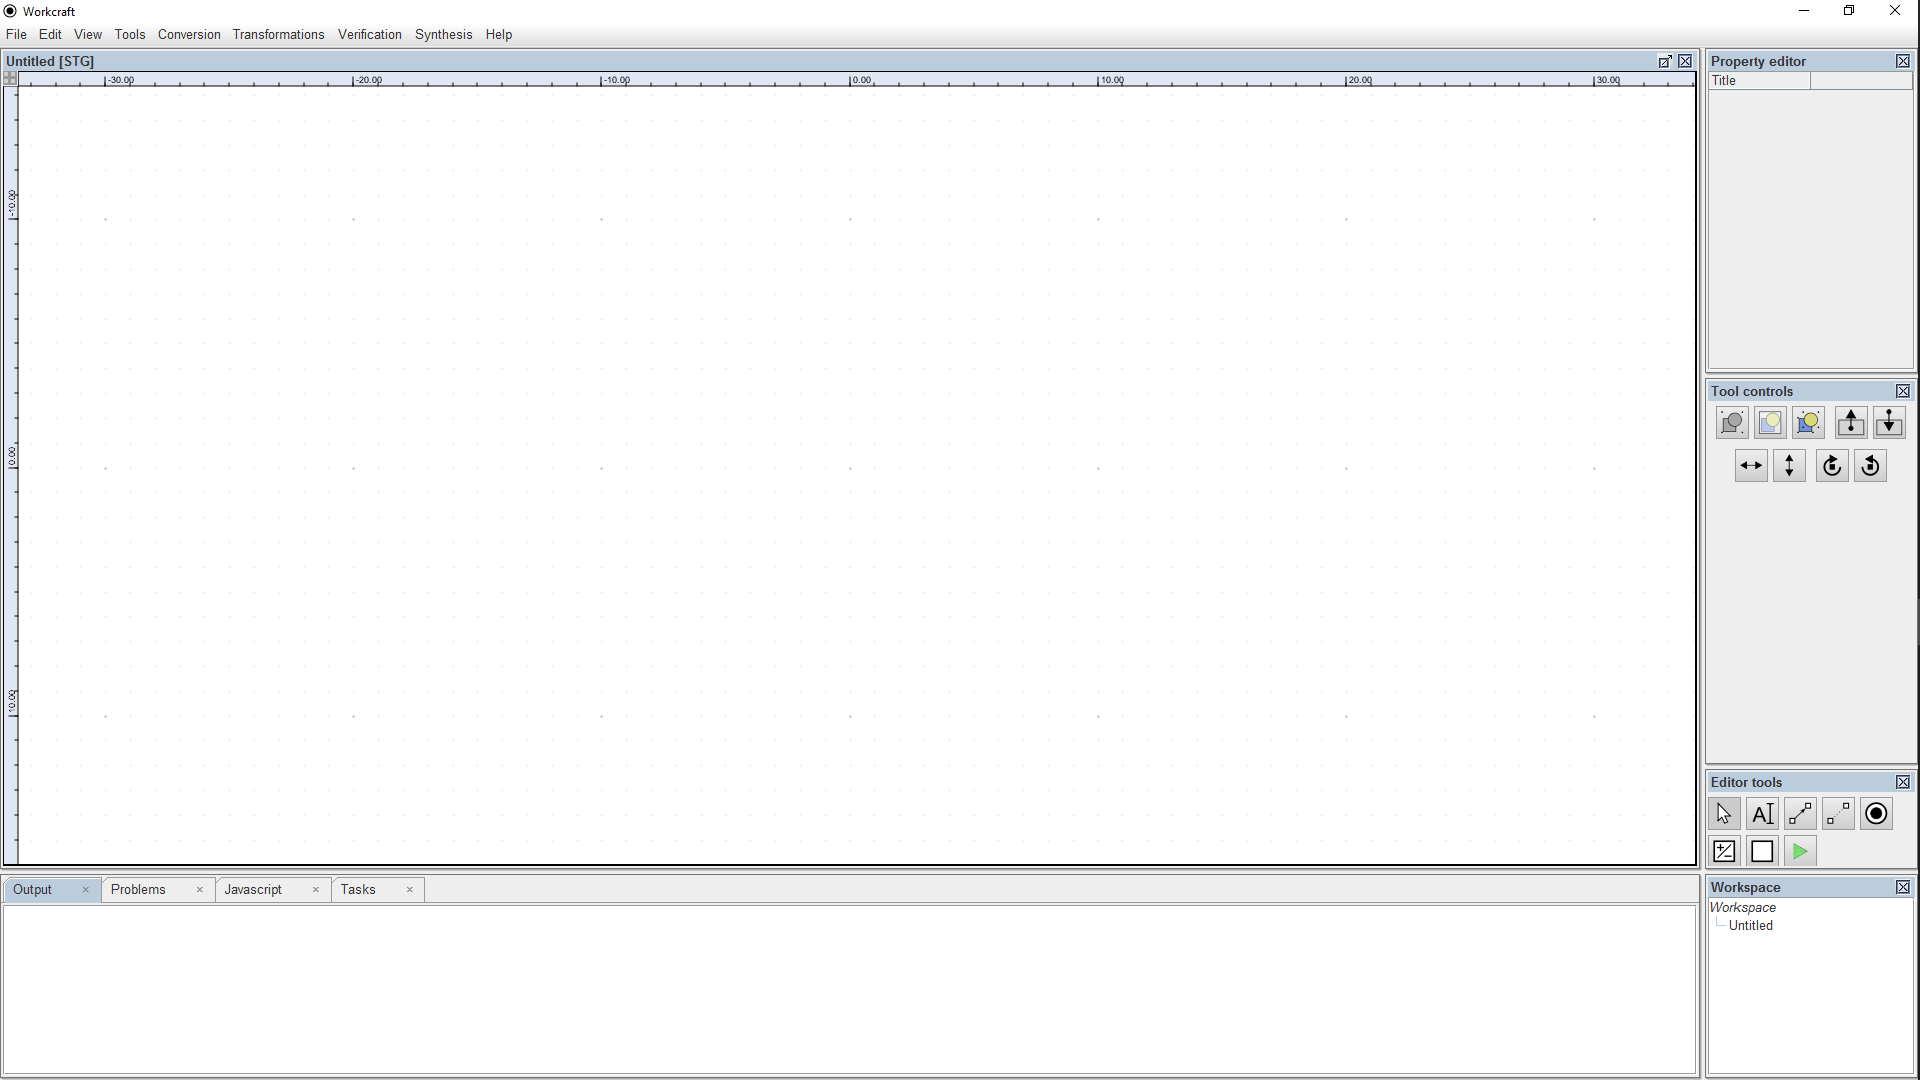
\includegraphics[scale=0.2]{images/new_stg_screenshot}
\par\end{centering}

\begin{centering}
\protect\caption{\label{fig:blank_stg_work}A new STG workspace}

\par\end{centering}

\end{figure}

Now, we can start translating concepts. To do this, first we need to open the concepts dialog.  This is done from the menu bar, by selecting the ``\emph{Conversion}'' menu, and then the 
``\emph{Translate concepts...}'' option. The concepts dialog will look as shown in Figure~\ref{fig:concepts_dialog_screenshot}.

\begin{figure}[H]
\begin{centering}
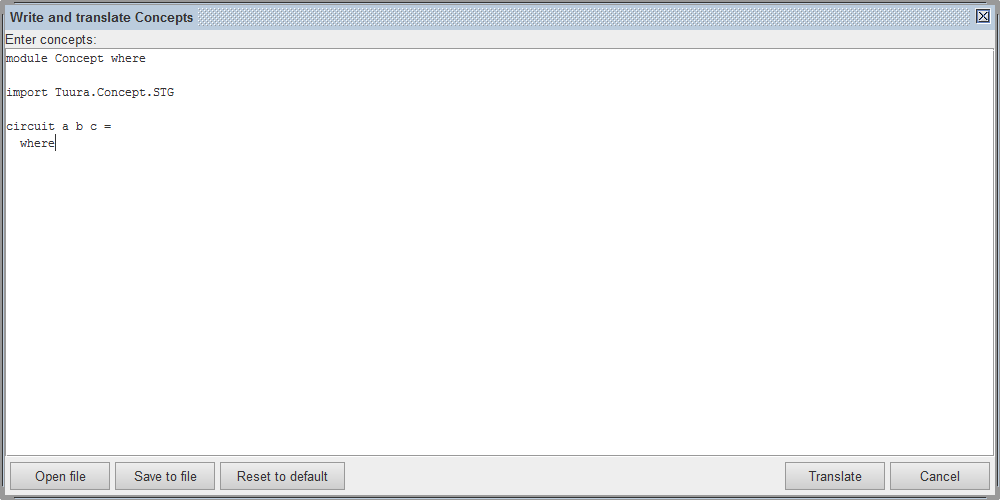
\includegraphics[scale=0.4]{images/concepts_dialog_screenshot}
\par\end{centering}

\begin{centering}
\protect\caption{\label{fig:concepts_dialog_screenshot}The concepts dialog.}

\par\end{centering}

\end{figure}

From within this dialog, one can write their own concepts, from the default template as shown in Figure~\ref{fig:concepts_dialog_screenshot}, or open an existing concepts file, with the  
\emph{.hs} extension. When satisfied with the concepts written, a user can choose to save the file, if not already saved, and then translate these concepts.

\begin{figure}[H]
\begin{centering}
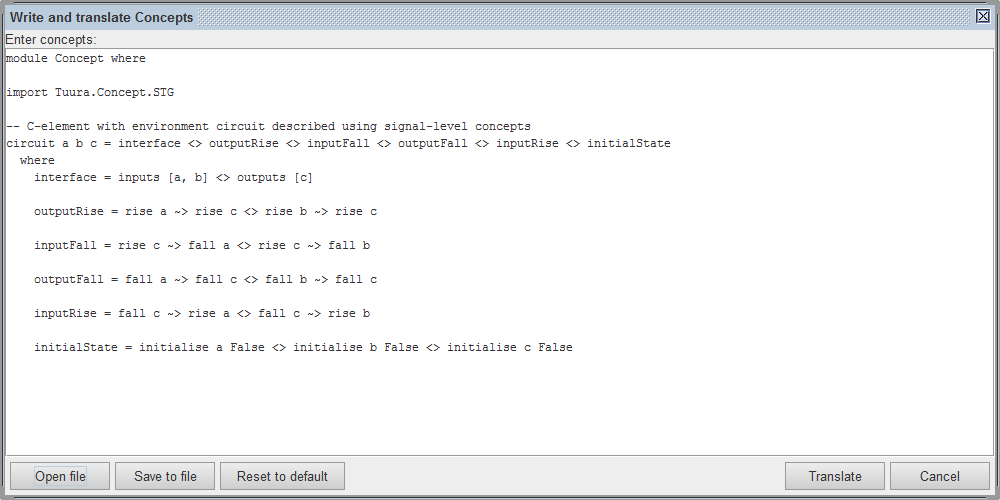
\includegraphics[scale=0.4]{images/concepts_dialog_Celement}
\par\end{centering}

\begin{centering}
\protect\caption{\label{fig:concepts_dialog_Celement}The concepts dialog with a concept file opened.}

\par\end{centering}

\end{figure}

Figure~\ref{fig:concepts_dialog_Celement} is the concepts dialog after we have opened the Celement with environment example, named ``\emph{Celement\_with\_env1.hs}'', from the 
concepts tool examples directory. Clicking translate at this point will produce an STG representation of these concepts in the workspace. 

\begin{figure}[H]
\begin{centering}
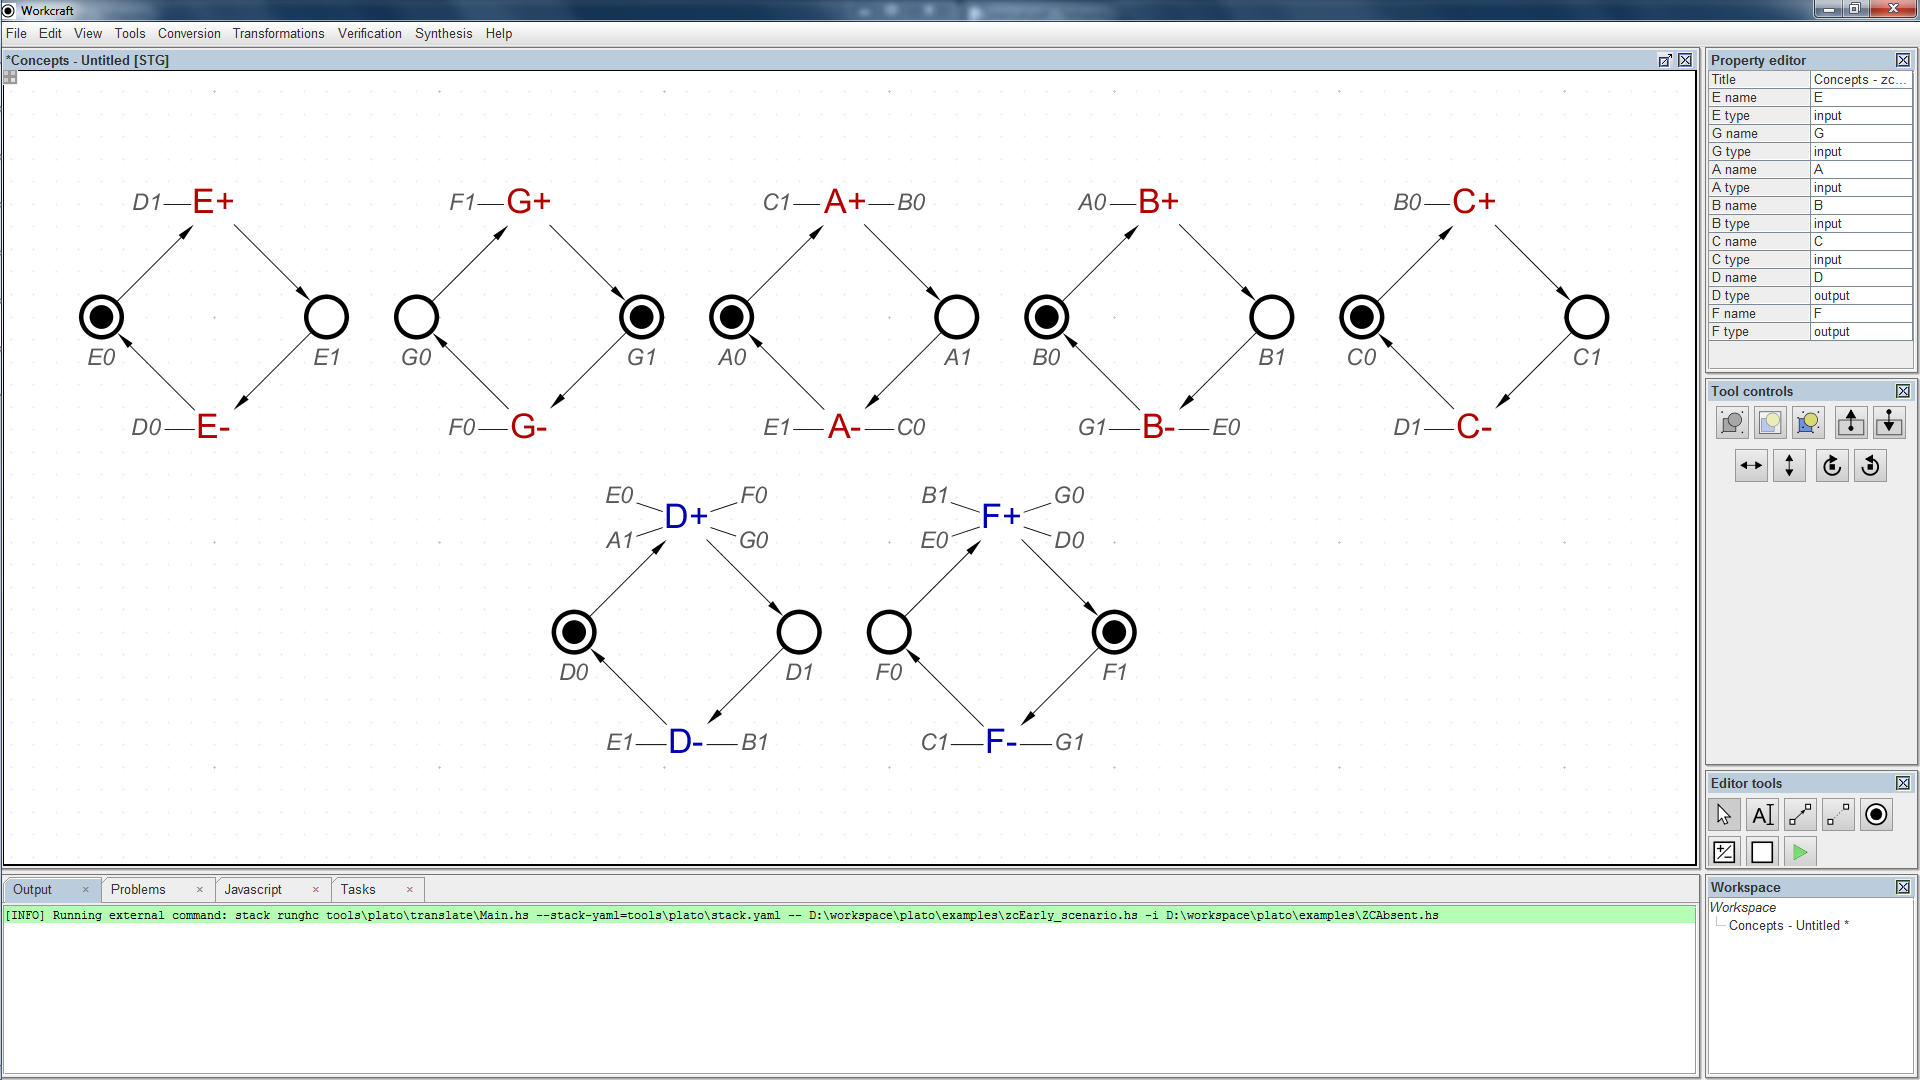
\includegraphics[scale=0.2]{images/concepts_translated}
\par\end{centering}

\begin{centering}
\protect\caption{\label{fig:concepts_translated}The STG produced from translating the concepts.}

\par\end{centering}

\end{figure}

The translated concepts will look similar to Figure~\ref{fig:concepts_translated}

Now, a user can choose to insert more concepts, make changes to this STG, and once they are satisfied with it, can then perform various functions on this STG. One can perform 
transformations, verifications, simulations and synthesis on this STG using the menus within this workspace now. Any further changes to this STG, based on the results of these operations 
can be made to this STG or to the concepts file. 

\section{Importing concepts directly}

It is also possible to import concepts directly from a file, without having to view the concepts first. This can be done from the ``\emph{File}'' menu, by selecting the ``\emph{Import...}'' 
option. 

\begin{figure}[H]
\begin{centering}
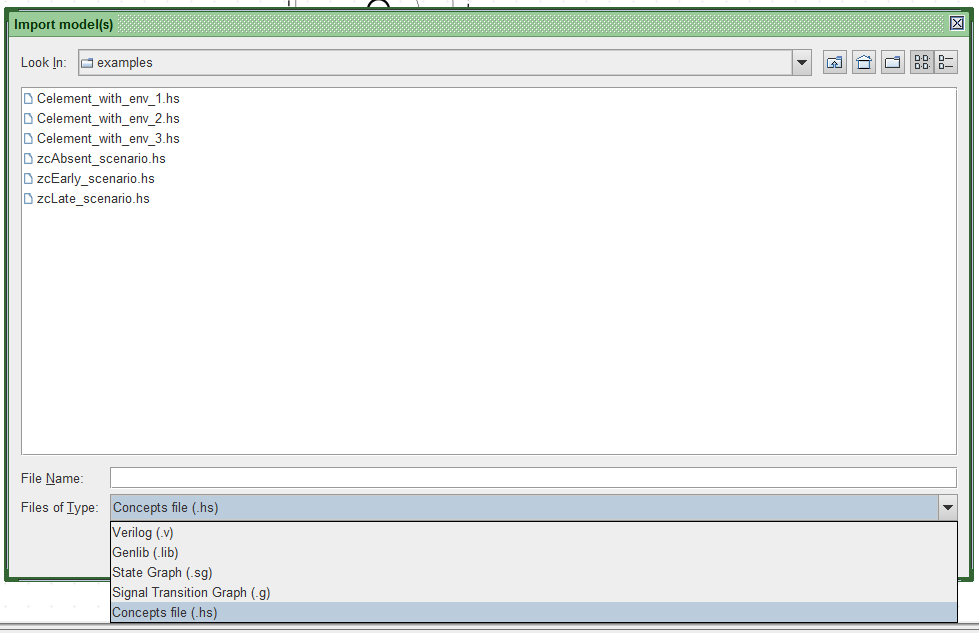
\includegraphics[scale=0.4]{images/import_menu_screenshot}
\par\end{centering}

\begin{centering}
\protect\caption{\label{fig:import_menu_screenshot}The STG produced from translating the concepts.}

\par\end{centering}

\end{figure}

When importing concepts using this menu, ensure to set the ``\emph{Files of Type}'' option to ``\emph{Concepts file (.hs)}'', as shown in Figure~\ref{fig:import_menu_screenshot}

\subsection{Errors}

If any errors are encountered during the translation process, \noun{Workcraft} will produce a helpful error message. This usually can tell you with more detail what the issue that is causing 
the error is, but will ask you to refer to \noun{Workcraft}'s console window for specific line numbers. These errors will include whether a signal has not been declared as an input or output,
a signal has not had it's initial state given, or even that the concepts tool has not been installed correctly. 

\section{Concepts file layout \label{sec:concepts_layout}}

\newpage
\bibliographystyle{unsrt}
\bibliography{manual_references}

\end{document}